\chapter{Parameter Study Capabilities}\label{ps}

\section{Overview}\label{ps:overview}

Dakota parameter studies explore the effect of parametric changes
within simulation models by computing response data sets at a
selection of points in the parameter space, yielding one type of
sensitivity analysis. (For a comparison with DACE-based sensitivity
analysis, see Section~\ref{dace:sa}.) The selection of points is
deterministic and structured, or user-specified, in each of the four
available parameter study methods:
\begin{itemize}
\item \textbf{Vector}: Performs a parameter study along a line between
  any two points in an $n$-dimensional parameter space, where the user
  specifies the number of steps used in the study.

\item \textbf{List}: The user supplies a list of points in an
  $n$-dimensional space where Dakota will evaluate response data from
  the simulation code.

\item \textbf{Centered}: Given a point in an $n$-dimensional parameter
  space, this method evaluates nearby points along the coordinate axes
  of the parameter space. The user selects the number of steps and the
  step size.

\item \textbf{Multidimensional}: Forms a regular lattice or hypergrid
  in an $n$-dimensional parameter space, where the user specifies the
  number of intervals used for each parameter.
\end{itemize}
More detail on these parameter studies is found in
Sections~\ref{ps:vector} through~\ref{ps:multidimensional} below.

When used in parameter studies, the response data sets are not linked
to any specific interpretation, so they may consist of any allowable
specification from the responses keyword block, i.e., objective and
constraint functions, least squares terms and constraints, or generic
response functions. This allows the use of parameter studies in
alternation with optimization, least squares, and uncertainty
quantification studies with only minor modification to the input
file. In addition, the response data sets may include gradients and
Hessians of the response functions, which will be catalogued by the
parameter study.  This allows for several different approaches to
``sensitivity analysis'': (1) the variation of function values over
parameter ranges provides a global assessment as to the sensitivity of
the functions to the parameters, (2) derivative information can be
computed numerically, provided analytically by the simulator, or both
(mixed gradients) in directly determining local sensitivity
information at a point in parameter space, and (3) the global and
local assessments can be combined to investigate the variation of
derivative quantities through the parameter space by computing
sensitivity information at multiple points.

In addition to sensitivity analysis applications, parameter studies
can be used for investigating nonsmoothness in simulation response
variations (so that models can be refined or finite difference step
sizes can be selected for computing numerical gradients),
interrogating problem areas in the parameter space, or performing
simulation code verification (verifying simulation robustness) through
parameter ranges of interest. A parameter study can also be used in
coordination with minimization methods as either a pre-processor (to
identify a good starting point) or a post-processor (for
post-optimality analysis).

Parameter study methods will iterate any combination of design,
uncertain, and state variables defined over continuous and discrete
domains into any set of responses (any function, gradient, and Hessian
definition). Parameter studies draw no distinction among the different
types of continuous variables (design, uncertain, or state) or among
the different types of response functions. They simply pass all of the
variables defined in the variables specification into the interface,
from which they expect to retrieve all of the responses defined in the
responses specification. As described in
Section~\ref{responses:active}, when gradient and/or Hessian
information is being catalogued in the parameter study, it is assumed
that derivative components will be computed with respect to all of the
\emph{continuous} variables (continuous design, continuous uncertain,
and continuous state variables) specified, since derivatives with
respect to discrete variables are assumed to be undefined.  The
specification of initial values or bounds is important for parameter
studies.

\subsection{Initial Values}\label{ps:overview:initial}

The vector and centered parameter studies use the initial values of
the variables from the \texttt{variables} keyword block as the
starting point and the central point of the parameter studies,
respectively. These parameter study starting values for design,
uncertain, and state variables are referenced in the following
sections using the identifier ``Initial Values.''

In the case of design variables, the \dakotakw{initial_point} is used,
and in the case of state variables, the \dakotakw{initial_state} is
used. In the case of uncertain variables, initial values not specified
by an \dakotakw{initial_point} are inferred from the distribution
specification: all uncertain initial values are set to their means,
correcting as needed.  For example, mean values for bounded normal and
bounded lognormal are repaired as needed to satisfy the specified
distribution bounds, mean values for discrete integer range
distributions are rounded down to the nearest integer, and mean values
for discrete set distributions are rounded to the nearest set
value. See the \dakotakw{variables}, \dakotakw{initial_point}, and
\dakotakw{initial_state} keywords in the Dakota Reference
Manual~\cite{RefMan} for additional details on default values.

\subsection{Bounds}\label{ps:overview:bounds}

The multidimensional parameter study uses the bounds of the variables
from the \texttt{variables} keyword block to define the range of
parameter values to study. In the case of design and state variables,
the \texttt{lower\_bounds} and \texttt{upper\_bounds} specifications
are used (see the Dakota Reference Manual~\cite{RefMan} for default
values when \texttt{lower\_bounds} or \texttt{upper\_bounds} are
unspecified). In the case of uncertain variables, these values are
either drawn or inferred from the distribution specification.
Distribution lower and upper bounds can be drawn directly from
required bounds specifications for uniform, loguniform, triangular,
and beta distributions, as well as from optional bounds specifications
for normal and lognormal.  Distribution bounds are implicitly defined
for histogram bin, histogram point, and interval variables (from the
extreme values within the bin/point/interval specifications) as well
as for binomial (0 to \texttt{num\_trials}) and hypergeometric (0 to
min(\texttt{num\_drawn},\texttt{num\_selected})) variables.  Finally,
distribution bounds are inferred for normal and lognormal if optional
bounds are unspecified, as well as for exponential, gamma, gumbel,
frechet, weibull, poisson, negative binomial, and geometric (which
have no bounds specifications); these bounds are [0, $\mu + 3 \sigma$]
for exponential, gamma, frechet, weibull, poisson, negative binomial,
geometric, and unspecified lognormal, and [$\mu - 3\sigma$, 
$\mu + 3\sigma$] for gumbel and unspecified normal.


\section{Vector Parameter Study}\label{ps:vector}

The vector parameter study computes response data sets at selected
intervals along an $n$-dimensional vector in parameter space. This
capability encompasses both single-coordinate parameter studies (to
study the effect of a single variable on a response set) as well as
multiple coordinate vector studies (to investigate the response
variations along some arbitrary vector; e.g., to investigate a
search direction failure).

Dakota's vector parameter study includes two possible specification
formulations which are used in conjunction with the Initial Values
(see Section~\ref{ps:overview:initial}) to define the vector and steps
of the parameter study:
\begin{small}
\begin{verbatim}
    final_point (vector of reals) and num_steps (integer)
    step_vector (vector of reals) and num_steps (integer)
\end{verbatim}
\end{small}

In both of these cases, the Initial Values are used as the parameter
study starting point and the specification selection above defines the
orientation of the vector and the increments to be evaluated along the
vector. In the former case, the vector from initial to final point is
partitioned by \texttt{num\_steps}, and in the latter case, the 
\texttt{step\_vector} is added \texttt{num\_steps} times.  In the case
of discrete range variables, both \texttt{final\_point} and 
\texttt{step\_vector} are specified in the actual values; and in the
case of discrete sets (integer or real), \texttt{final\_point} is
specified in the actual values but \texttt{step\_vector} must instead
specify index offsets for the (ordered, unique) set.  In all cases,
the number of evaluations is \texttt{num\_steps}+1. Two examples are
included below:

Three continuous parameters with initial values of (1.0, 1.0, 1.0), 
\texttt{num\_steps} = 4, and either \texttt{final\_point} = 
(1.0, 2.0, 1.0) or \texttt{step\_vector} = (0, .25, 0):
\begin{small}
\begin{verbatim}
    Parameters for function evaluation 1:
                          1.0000000000e+00 c1   
                          1.0000000000e+00 c2   
                          1.0000000000e+00 c3   
    Parameters for function evaluation 2:
                          1.0000000000e+00 c1   
                          1.2500000000e+00 c2   
                          1.0000000000e+00 c3   
    Parameters for function evaluation 3:
                          1.0000000000e+00 c1   
                          1.5000000000e+00 c2   
                          1.0000000000e+00 c3   
    Parameters for function evaluation 4:
                          1.0000000000e+00 c1   
                          1.7500000000e+00 c2   
                          1.0000000000e+00 c3   
    Parameters for function evaluation 5:
                          1.0000000000e+00 c1   
                          2.0000000000e+00 c2   
                          1.0000000000e+00 c3   
\end{verbatim}
\end{small}

Two continuous parameters with initial values of (1.0, 1.0), one
discrete range parameter with initial value of 5, one discrete real
set parameter with set values of (10., 12., 18., 30., 50.) and initial
value of 10., \texttt{num\_steps} = 4, and either \texttt{final\_point}
= (2.0, 1.4, 13, 50.) or \texttt{step\_vector} = (.25, .1, 2, 1):
\begin{small}
\begin{verbatim}
    Parameters for function evaluation 1:
                          1.0000000000e+00 c1
                          1.0000000000e+00 c2
                                         5 di1
                          1.0000000000e+01 dr1
    Parameters for function evaluation 2:
                          1.2500000000e+00 c1   
                          1.1000000000e+00 c2   
                                         7 di1
                          1.2000000000e+01 dr1
    Parameters for function evaluation 3:
                          1.5000000000e+00 c1   
                          1.2000000000e+00 c2   
                                         9 di1
                          1.8000000000e+01 dr1
    Parameters for function evaluation 4:
                          1.7500000000e+00 c1   
                          1.3000000000e+00 c2   
                                        11 di1
                          3.0000000000e+01 dr1
    Parameters for function evaluation 5:
                          2.0000000000e+00 c1   
                          1.4000000000e+00 c2   
                                        13 di1
                          5.0000000000e+01 dr1
\end{verbatim}
\end{small}

An example using a vector parameter study is described in 
Section~\ref{ps:example:vector}.

\section{List Parameter Study}\label{ps:list}

The list parameter study computes response data sets at selected
points in parameter space. These points are explicitly specified by
the user and are not confined to lie on any line or surface. Thus,
this parameter study provides a general facility that supports the
case where the desired set of points to evaluate does not fit the
prescribed structure of the vector, centered, or multidimensional
parameter studies.

The user input consists of a \texttt{list\_of\_points} specification
which lists the requested parameter sets in succession. The list
parameter study simply performs a simulation for the first parameter
set (the first $n$ entries in the list), followed by a simulation for
the next parameter set (the next $n$ entries), and so on, until the
list of points has been exhausted. Since the Initial Values will not
be used, they need not be specified.  In the case of discrete range or
discrete set variables, list values are specified using the actual
values (not set indices).

An example specification that would result in the same parameter sets
as in the second example in Section~\ref{ps:vector} would be:
\begin{small}
\begin{verbatim}
    list_of_points = 1.0  1.0  5 10.
                     1.25 1.1  7 12.
                     1.5  1.2  9 18.
                     1.75 1.3 11 30.
                     2.0  1.4 13 50.
\end{verbatim}
\end{small}

For convenience, the points for evaluation in a list parameter study
may instead be specified via the \dakotakw{import_points_file}
specification, e.g., {\tt import\_points\_file 'listpstudy.dat'},
where the file \path{listpstudy.dat} may be in freeform or annotated
format~\ref{input:tabularformat}.  The ordering of the points is in
input specification order, with both active and inactive variables by
default.

\section{Centered Parameter Study}\label{ps:centered}

The centered parameter study executes multiple coordinate-based
parameter studies, one per parameter, centered about the specified
Initial Values. This is useful for investigation of function contours
in the vicinity of a specific point. For example, after computing an
optimum design, this capability could be used for post-optimality
analysis in verifying that the computed solution is actually at a
minimum or constraint boundary and in investigating the shape of this
minimum or constraint boundary.

This method requires \texttt{step\_vector} (list of reals) and
\texttt{steps\_per\_variable} (list of integers) specifications, where 
the former specifies the size of the increments per variable (employed
sequentially, not all at once as for the vector study in
Section~\ref{ps:vector}) and the latter specifies the number of
increments per variable (employed sequentially, not all at once) for
each of the positive and negative step directions.  As for the vector
study described in Section~\ref{ps:vector}, \texttt{step\_vector}
includes actual variable steps for continuous and discrete range
variables, but employs index offsets for discrete set variables
(integer or real).

For example, with Initial Values of (1.0, 1.0), a \texttt{step\_vector} 
of (0.1, 0.1), and a \texttt{steps\_per\_variable} of (2, 2), the 
center point is evaluated followed by four function evaluations (two 
negative deltas and two positive deltas) per variable:
\begin{small}
\begin{verbatim}
    Parameters for function evaluation 1:
                          1.0000000000e+00 d1
                          1.0000000000e+00 d2
    Parameters for function evaluation 2:
                          8.0000000000e-01 d1
                          1.0000000000e+00 d2
    Parameters for function evaluation 3:
                          9.0000000000e-01 d1
                          1.0000000000e+00 d2
    Parameters for function evaluation 4:
                          1.1000000000e+00 d1
                          1.0000000000e+00 d2
    Parameters for function evaluation 5:
                          1.2000000000e+00 d1
                          1.0000000000e+00 d2
    Parameters for function evaluation 6:
                          1.0000000000e+00 d1
                          8.0000000000e-01 d2
    Parameters for function evaluation 7:
                          1.0000000000e+00 d1
                          9.0000000000e-01 d2
    Parameters for function evaluation 8:
                          1.0000000000e+00 d1
                          1.1000000000e+00 d2
    Parameters for function evaluation 9:
                          1.0000000000e+00 d1
                          1.2000000000e+00 d2
\end{verbatim}
\end{small}

This set of points in parameter space is depicted in Figure~\ref{ps:figure01}.
\begin{figure}
  \centering
  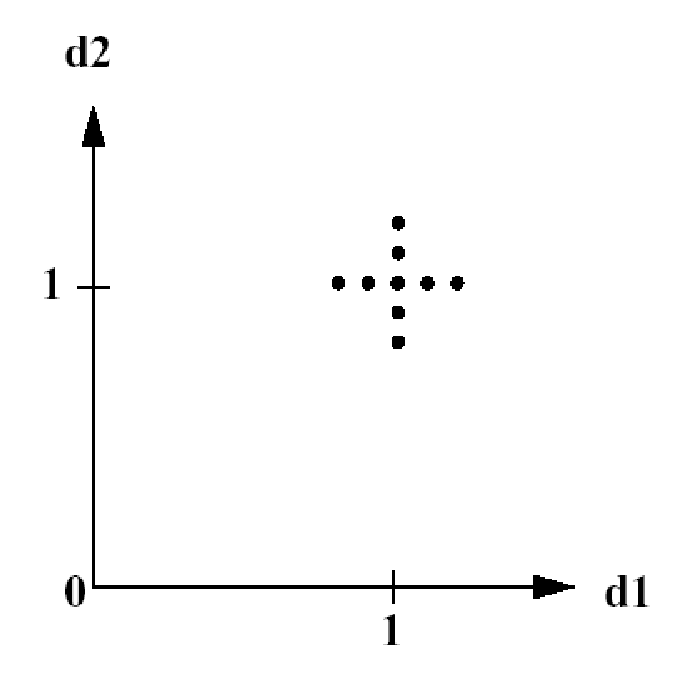
\includegraphics[scale=0.5]{images/centered_pstudy}
  \caption{Example centered parameter study.}
  \label{ps:figure01}
\end{figure}


\section{Multidimensional Parameter Study}\label{ps:multidimensional}

The multidimensional parameter study computes response data sets for
an $n$-dimensional hypergrid of points. Each variable is partitioned
into equally spaced intervals between its upper and lower bounds (see
Section~\ref{ps:overview:bounds}), and each combination of the values
defined by these partitions is evaluated.  As for the vector and
centered studies described in Sections~\ref{ps:vector}
and~\ref{ps:centered}, partitioning occurs using the actual variable
values for continuous and discrete range variables, but occurs within
the space of valid indices for discrete set variables (integer or
real).  The number of function evaluations performed in the study is:
\begin{equation}
  \prod_{i=1}^{n}(\hbox{\texttt{partitions}}_{i}+1)
  \label{ps:equation01}
\end{equation}

The partitions information is specified using the \texttt{partitions}
specification, which provides an integer list of the number of
partitions for each variable (i.e., \texttt{partitions}$_{i}$). Since
the Initial Values will not be used, they need not be specified.

In a two variable example problem with \texttt{d1} $\in$ [0,2] and 
\texttt{d2} $\in$ [0,3] (as defined by the upper and lower bounds 
from the variables specification) and with \texttt{partitions} =
(2,3), the interval [0,2] is divided into two equal-sized partitions
and the interval [0,3] is divided into three equal-sized partitions. 
This two-dimensional grid, shown in Figure~\ref{ps:figure02}, would 
result in the following twelve function evaluations:
\begin{figure}
  \centering
  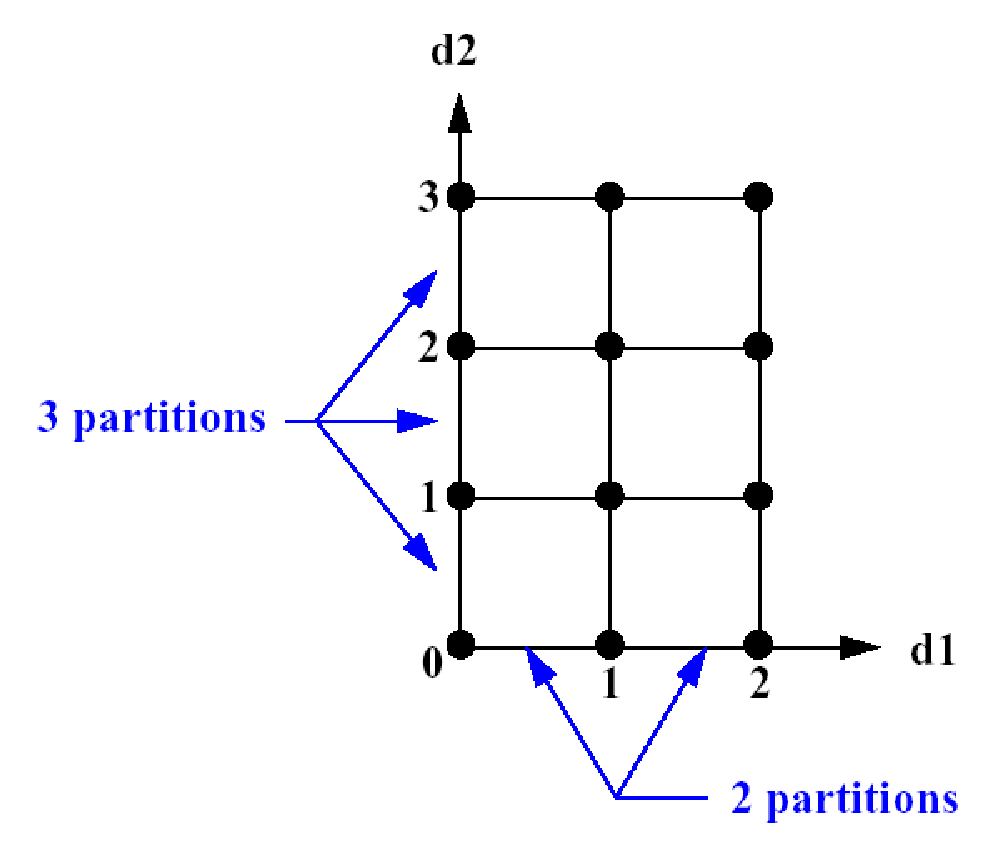
\includegraphics[scale=0.5]{images/multi_d_pstudy}
  \caption{Example multidimensional parameter study}
  \label{ps:figure02}
\end{figure}

\begin{small}
\begin{verbatim}
    Parameters for function evaluation 1:
                          0.0000000000e+00 d1   
                          0.0000000000e+00 d2   
    Parameters for function evaluation 2:
                          1.0000000000e+00 d1   
                          0.0000000000e+00 d2   
    Parameters for function evaluation 3:
                          2.0000000000e+00 d1   
                          0.0000000000e+00 d2   
    Parameters for function evaluation 4:
                          0.0000000000e+00 d1   
                          1.0000000000e+00 d2   
    Parameters for function evaluation 5:
                          1.0000000000e+00 d1   
                          1.0000000000e+00 d2   
    Parameters for function evaluation 6:
                          2.0000000000e+00 d1   
                          1.0000000000e+00 d2   
    Parameters for function evaluation 7:
                          0.0000000000e+00 d1   
                          2.0000000000e+00 d2   
    Parameters for function evaluation 8:
                          1.0000000000e+00 d1   
                          2.0000000000e+00 d2   
    Parameters for function evaluation 9:
                          2.0000000000e+00 d1   
                          2.0000000000e+00 d2   
    Parameters for function evaluation 10:
                          0.0000000000e+00 d1   
                          3.0000000000e+00 d2   
    Parameters for function evaluation 11:
                          1.0000000000e+00 d1   
                          3.0000000000e+00 d2   
    Parameters for function evaluation 12:
                          2.0000000000e+00 d1   
                          3.0000000000e+00 d2
\end{verbatim}
\end{small}

The first example shown in this User's Manual is a multi-dimensional
parameter study. See Section~\ref{tutorial:examples:param_study}.

\section{Parameter Study Usage Guidelines}\label{ps:usage}

Parameter studies, classical design of experiments (DOE),
design/analysis of computer experiments (DACE), and sampling methods
share the purpose of exploring the parameter space.  Parameter Studies
are recommended for simple studies with defined, repetitive structure.
A local sensitivity analysis or an assessment of the
smoothness of a response function is best addressed with a vector or
centered parameter study. A multi-dimensional parameter 
study may be used to generate grid points for plotting response surfaces.
For guidance on DACE and sampling methods, in contrast to parameter 
studies, see Section~\ref{dace:usage} and especially Table~\ref{dace:usage:table},
which clarifies the different purposes of the method types.
 
\section{Example: Vector Parameter Study with Rosenbrock}\label{ps:example:vector}

This section demonstrates a vector parameter study on the Rosenbrock 
test function described in Section~\ref{tutorial:examples:rosenbrock}.  
An example of multidimensional parameter study is shown in 
Section~\ref{tutorial:examples:param_study}.

A vector parameter study is a study between any 
two design points in an \emph{n}-dimensional parameter space.
An input file for the vector parameter study is shown in Figure~
\ref{additional:rosenbrock_vector}. The primary differences
between this input file and the input file for the multidimensional
parameter study are found in the
\emph{variables} and \emph{method} sections. In the variables section,
the keywords for the bounds are removed and replaced with the keyword
\texttt{initial\_point} that specifies the starting point for the
parameter study. In the method section, the
\texttt{vector\_parameter\_study} keyword is used. The
\texttt{final\_point} keyword indicates the stopping point for the
parameter study, and \texttt{num\_steps} specifies the number of steps
taken between the initial and final points in the parameter study.

\begin{figure}[ht!]
  \centering
  \begin{bigbox}
    \begin{small}
      \verbatimtabinput[8]{../../../test/examples-users/rosen_ps_vector.in}
    \end{small}
  \end{bigbox}
  \caption{Rosenbrock vector parameter study example: the Dakota input
    file -- see
    \protect\path{dakota/share/dakota/examples/users/rosen_ps_vector.in}
  }
  \label{additional:rosenbrock_vector}
\end{figure}

Figure~\ref{additional:rosenbrock_vector_graphics}(a) shows the legacy
X Windows-based graphics output created by Dakota, which can be useful
for visualizing the
results. Figure~\ref{additional:rosenbrock_vector_graphics}(b) shows
the locations of the 11 sample points generated in this study.  It is
evident from these figures that the parameter study starts within the
banana-shaped valley, marches up the side of the hill, and then
returns to the valley.

\begin{figure}[htp!]
  \centering
  \begin{tabular}{c}
  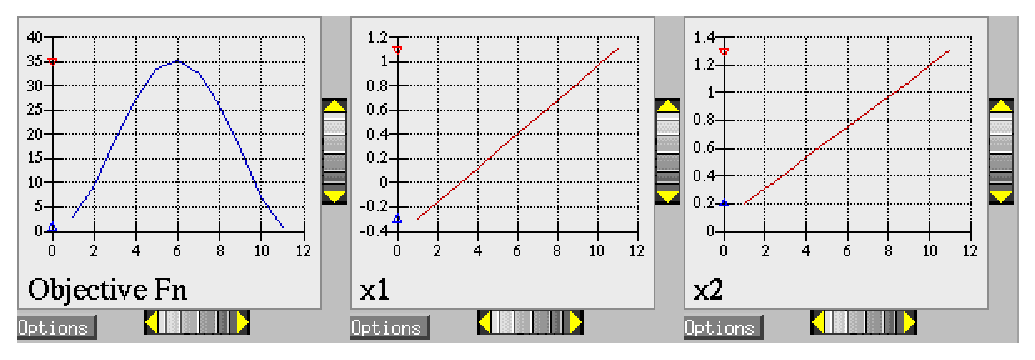
\includegraphics[width=\textwidth]{images/dak_graphics_vector}\\
  (a)\\
  \qquad\\
  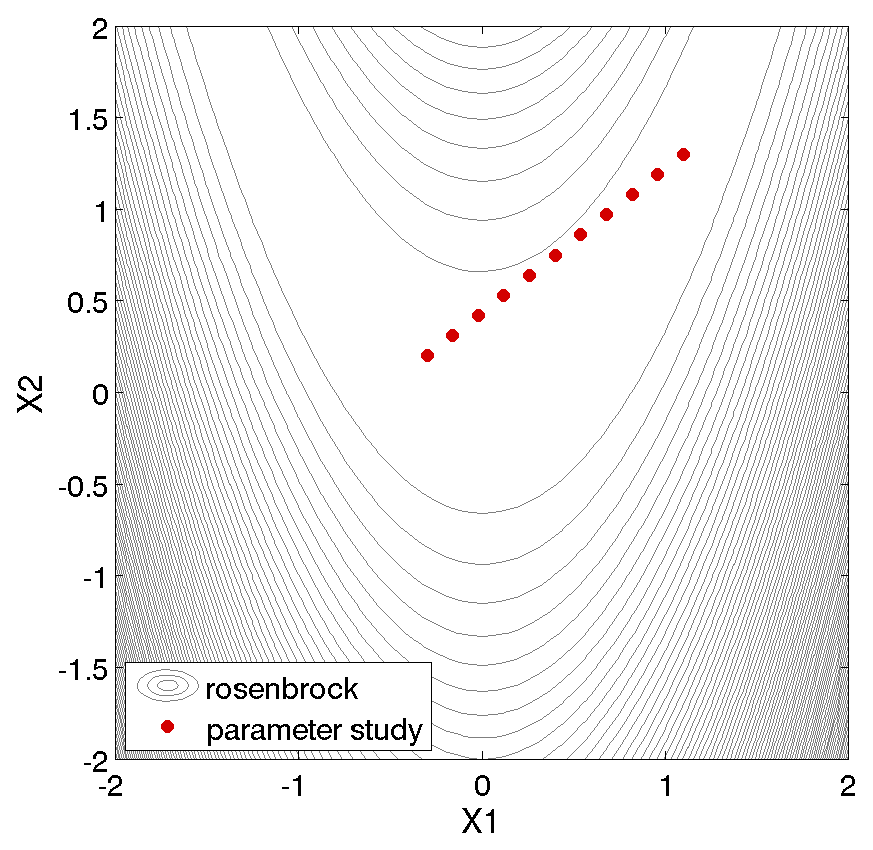
\includegraphics[height=2.5in]{images/rosen_vect_pts} \\
  (b)
  \end{tabular}
  \caption{Rosenbrock vector parameter study example: (a) screen
    capture of the Dakota graphics and (b) location of the design
    points (dots) evaluated.}
  \label{additional:rosenbrock_vector_graphics}
\end{figure}
